\section{Bagian II --- Landasan Teori, Desain Arsitektur, dan Formulasi Matematika}

\subsection{Protokol eksperimen terstandarisasi}
Seluruh model dilatih pada \textbf{Fashion-MNIST} (28$\times$28 grayscale, 10 kelas). Kedua split bawaan
\texttt{torchvision} (60.000 + 10.000) digabung menjadi 70.000 citra lalu dipermutasi dengan
\texttt{torch.Generator().manual\_seed(42)} menjadi \textbf{56.000 train / 7.000 validation / 7.000 test} (80/10/10).
Indeks split identik untuk semua model; \texttt{random}, \texttt{numpy}, dan \texttt{torch} di-seed 42 sebelum setiap
training. \texttt{batch\_size}=128, \texttt{shuffle=True} pada train dan \texttt{shuffle=False} pada val/test.
Model AE/Sparse AE/VAE memakai piksel $[0,1]$ (keluaran Sigmoid); GAN, DCGAN, dan DDPM memakai $[-1,1]$ (Tanh)
dan dikonversi kembali ke $[0,1]$ sebelum evaluasi. Seluruh eksperimen dijalankan pada CPU 2-core (tanpa GPU),
sehingga ukuran model dan jumlah epoch dipilih agar seluruh pipeline dapat direproduksi dalam beberapa jam.

\subsection{Diagram skematik arsitektur}
Figur 0 merangkum ketujuh arsitektur. Encoder Vanilla AE, Sparse AE, VAE, dan MLP Classifier
sengaja dibuat identik ($784\!\to\!256\!\to\!64$) sehingga perbedaan perilaku hanya berasal dari \emph{fungsi objektif}.

\begin{figure}[h]
\centering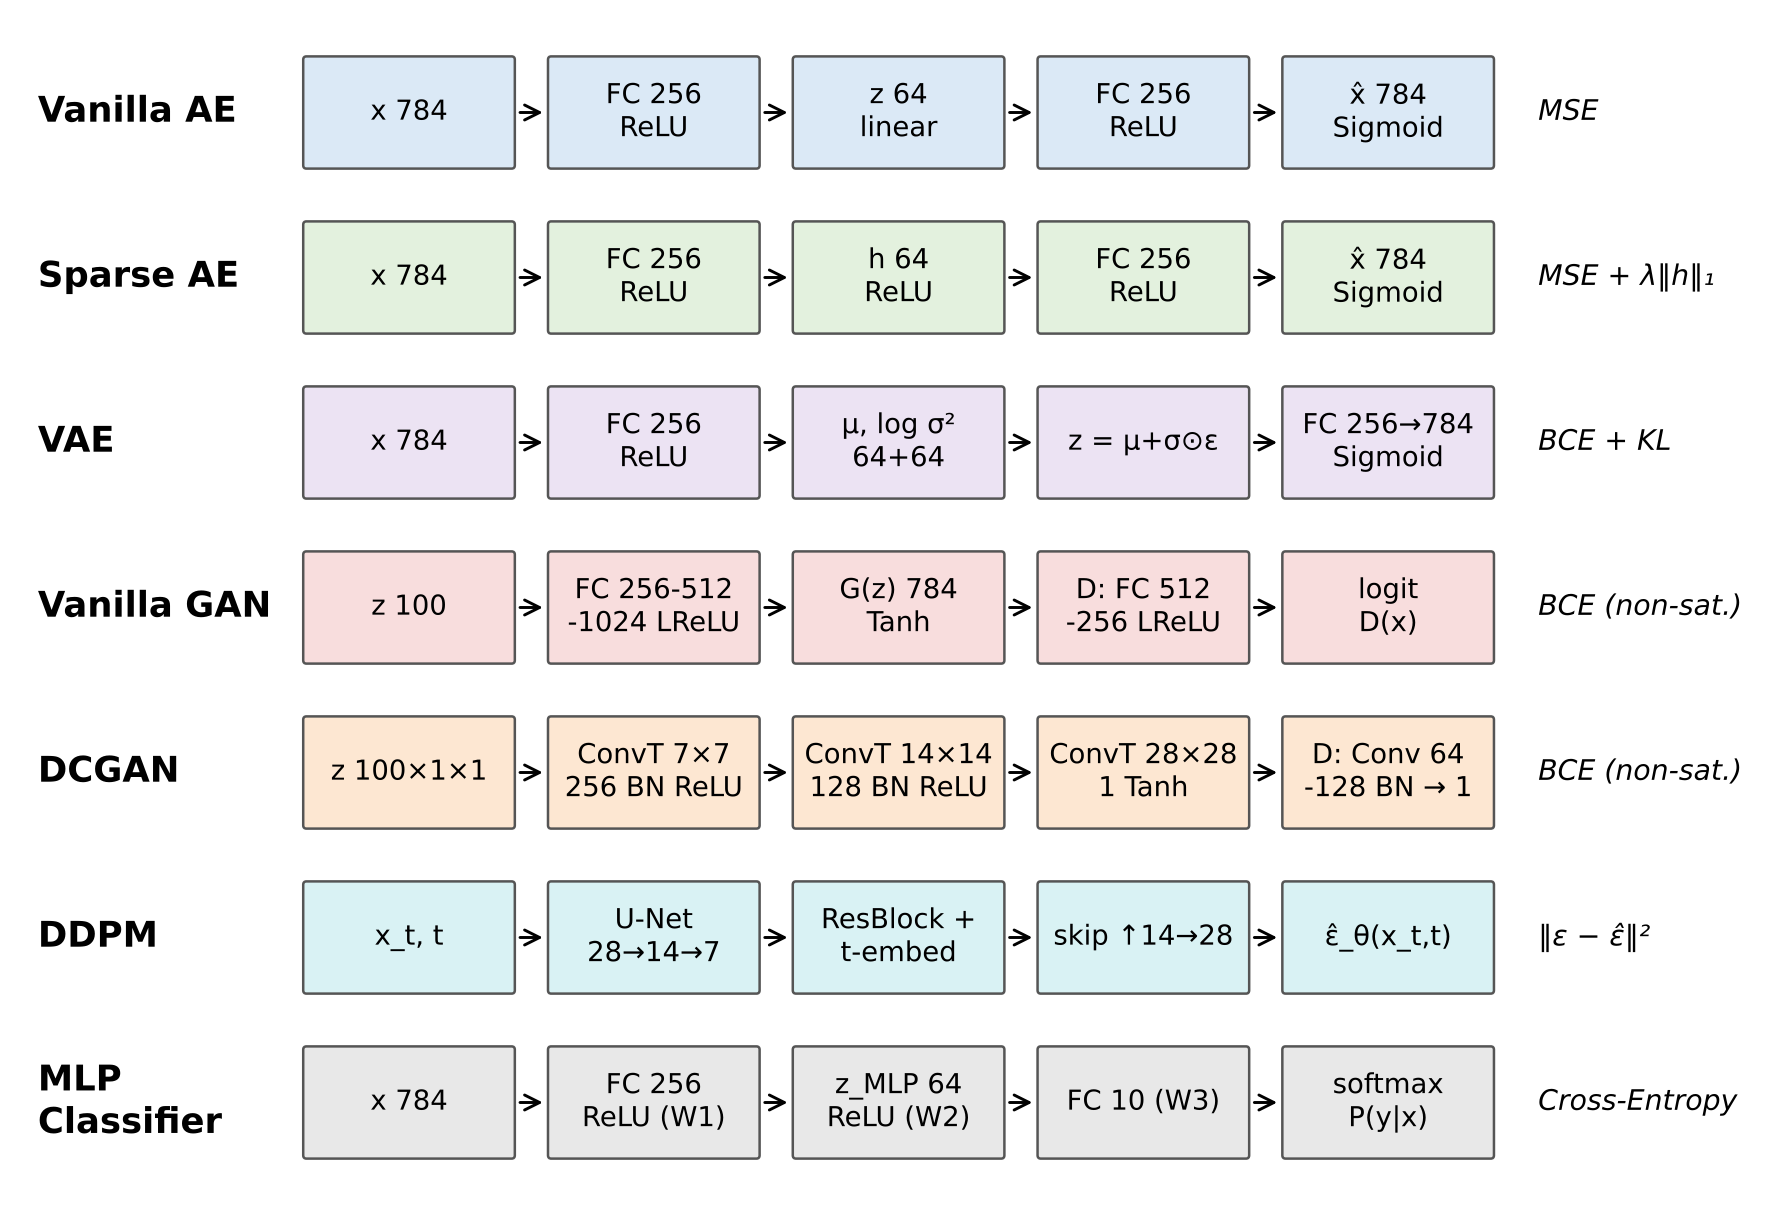
\includegraphics[width=0.93\linewidth]{../outputs/figures/fig0_arsitektur.png}
\caption{\textbf{Figur 0.} Skema arsitektur ketujuh model (blok = lapisan, teks miring = fungsi loss). FC = fully connected,
ConvT = transposed convolution, BN = BatchNorm, LReLU = LeakyReLU(0,2).}
\label{fig:arch}
\end{figure}

\subsection{Tabel konfigurasi parameter}
\begin{table}[h]
\centering\small
\caption{Konfigurasi arsitektur dan optimasi. Jumlah parameter dihitung dari model terlatih.}
\label{tab:config}
\begin{tabular}{@{}lp{4.6cm}cccc@{}}
\toprule
Model & Lapisan & Laten & Aktivasi & Optimizer, LR & Epoch \\
\midrule
Vanilla AE & FC 784-256-64-256-784 & 64 (linear) & ReLU / Sigmoid & Adam, $10^{-3}$ & 30 \\
Sparse AE & idem, $\lambda=10^{-4}$ & 64 (ReLU) & ReLU / Sigmoid & Adam, $10^{-3}$ & 30 \\
VAE & FC 784-256-($\mu$,$\log\sigma^2$)-256-784 & 64 & ReLU / Sigmoid & Adam, $10^{-3}$ & 30 \\
Vanilla GAN & G: FC 100-256-512-1024-784; D: FC 784-512-256-1 & 100 & LReLU / Tanh & Adam, $2\!\cdot\!10^{-4}$, $\beta_1\!=\!0{,}5$ & 50 \\
DCGAN & G: ConvT 7$\times$7$\times$256$\to$14$\times$14$\times$128$\to$28$\times$28; D: Conv 64-128-1 (stride 2) & 100 & ReLU+BN / LReLU / Tanh & Adam, $2\!\cdot\!10^{-4}$, $\beta_1\!=\!0{,}5$ & 20 \\
DDPM & U-Net 3 level (32/64/128), ResBlock+GroupNorm, sinusoidal $t$-embed; $T=1000$, $\beta_t$ linier $10^{-4}\!\to\!0{,}02$, EMA 0,999 & 784 & SiLU & Adam, $2\!\cdot\!10^{-4}$ & 12 \\
MLP Classifier & FC 784-256-64-10 & 64 & ReLU / Softmax & Adam, $10^{-3}$ & 25 \\
\bottomrule
\end{tabular}
\end{table}

\noindent\textbf{Catatan desain.} (i) Uji awal 3 epoch menunjukkan Vanilla AE dengan kode ReLU tanpa penalti
kehilangan $\approx$20/64 unit (\emph{dead units}); karena itu Vanilla AE memakai kode laten linear (representasi padat).
(ii) Sparse AE memakai kode ReLU agar penalti L1 menghasilkan nol eksak; $\lambda=10^{-3}$ membuat seluruh unit mati
(kolaps), sehingga dipilih $\lambda=10^{-4}$. (iii) Generator GAN/DCGAN memakai prior berdimensi 100 dan inisialisasi
DCGAN $\mathcal{N}(0;0{,}02)$.

\subsection{Formulasi matematika fungsi loss}
\textbf{Vanilla AE.} Encoder $f_\phi$ dan decoder $g_\theta$ meminimalkan galat rekonstruksi
\begin{equation}
\mathcal{L}_{\text{AE}}=\frac{1}{N}\sum_{i=1}^{N}\frac{1}{D}\lVert x_i-g_\theta(f_\phi(x_i))\rVert_2^2 .
\end{equation}
\textbf{Sparse AE.} Ditambahkan penalti L1 pada kode $h=\mathrm{ReLU}(f_\phi(x))$:
\begin{equation}
\mathcal{L}_{\text{SAE}}=\mathcal{L}_{\text{AE}}+\lambda\,\frac{1}{N}\sum_i\lVert h_i\rVert_1 ,\qquad \lambda=10^{-4}.
\end{equation}
Penalti L1 adalah relaksasi konveks dari norma $\ell_0$; gradiennya konstan ($\lambda\,\mathrm{sign}(h)$) sehingga
mendorong unit yang kurang berguna tepat ke nol.

\textbf{VAE.} Dengan posterior aproksimasi $q_\phi(z|x)=\mathcal{N}(\mu_\phi(x),\mathrm{diag}\,\sigma^2_\phi(x))$ dan
prior $p(z)=\mathcal{N}(0,I)$, VAE memaksimalkan ELBO $\log p_\theta(x)\ge \mathbb{E}_{q}[\log p_\theta(x|z)]-D_{\text{KL}}(q_\phi(z|x)\Vert p(z))$.
Dengan likelihood Bernoulli dan KL tertutup, loss per sampel:
\begin{equation}
\mathcal{L}_{\text{VAE}}=-\sum_{j=1}^{784}\big[x_j\log\hat{x}_j+(1-x_j)\log(1-\hat{x}_j)\big]
-\frac12\sum_{k=1}^{64}\big(1+\log\sigma_k^2-\mu_k^2-\sigma_k^2\big),
\end{equation}
dengan $z=\mu+\sigma\odot\varepsilon$, $\varepsilon\sim\mathcal{N}(0,I)$ (\emph{reparameterization trick}).

\textbf{Vanilla GAN dan DCGAN.} Generator $G$ dan diskriminator $D$ memainkan permainan minimax
\begin{equation}
\min_G\max_D\;V(D,G)=\mathbb{E}_{x\sim p_{\text{data}}}[\log D(x)]+\mathbb{E}_{z\sim\mathcal{N}(0,I)}[\log(1-D(G(z)))].
\end{equation}
Untuk $D$ optimal $D^*(x)=\frac{p_{\text{data}}(x)}{p_{\text{data}}(x)+p_g(x)}$ sehingga $V(D^*,G)=-\log 4+2\,D_{\text{JS}}(p_{\text{data}}\Vert p_g)$.
Dalam implementasi, $D$ meminimalkan $\mathcal{L}_D=-\mathbb{E}[\log D(x)]-\mathbb{E}[\log(1-D(G(z)))]$ dan $G$ memakai
bentuk \emph{non-saturating} $\mathcal{L}_G=-\mathbb{E}[\log D(G(z))]$ (Goodfellow dkk., 2014). DCGAN memakai loss
yang sama; yang berbeda adalah \emph{inductive bias} arsitekturnya (konvolusi, BatchNorm, strided conv tanpa pooling).

\textbf{DDPM.} Proses maju menambahkan derau Gaussian:
$q(x_t|x_0)=\mathcal{N}(\sqrt{\bar\alpha_t}\,x_0,(1-\bar\alpha_t)I)$ dengan $\alpha_t=1-\beta_t$, $\bar\alpha_t=\prod_{s\le t}\alpha_s$.
Jaringan $\varepsilon_\theta$ dilatih dengan objektif \emph{supervised noise prediction}
\begin{equation}
\mathcal{L}_{\text{simple}}=\mathbb{E}_{t\sim\mathcal{U}\{1..T\},\,x_0,\,\varepsilon\sim\mathcal{N}(0,I)}
\big\lVert\varepsilon-\varepsilon_\theta(\sqrt{\bar\alpha_t}x_0+\sqrt{1-\bar\alpha_t}\,\varepsilon,\;t)\big\rVert_2^2 ,
\end{equation}
dan sampling dilakukan dengan $T=1000$ langkah reverse
$x_{t-1}=\frac{1}{\sqrt{\alpha_t}}\big(x_t-\frac{1-\alpha_t}{\sqrt{1-\bar\alpha_t}}\varepsilon_\theta(x_t,t)\big)+\sigma_t z$,
$\sigma_t^2=\tilde\beta_t=\frac{1-\bar\alpha_{t-1}}{1-\bar\alpha_t}\beta_t$.

\textbf{MLP Classifier.} $p(y|x)=\mathrm{softmax}(W_3\,z_{\text{MLP}}+b_3)$ dengan
$z_{\text{MLP}}=\mathrm{ReLU}(W_2\,\mathrm{ReLU}(W_1x+b_1)+b_2)\in\mathbb{R}^{64}$ dan
$\mathcal{L}_{\text{CE}}=-\frac1N\sum_i\log p(y_i|x_i)$.

\subsection{Metrik evaluasi}
MSE dan PSNR $=10\log_{10}(1/\text{MSE})$ dihitung per citra lalu dirata-rata; SSIM memakai
\texttt{skimage} (\texttt{data\_range}=1). FID $=\lVert\mu_r-\mu_g\rVert^2+\mathrm{Tr}(\Sigma_r+\Sigma_g-2(\Sigma_r\Sigma_g)^{1/2})$
dihitung dari fitur pool3 InceptionV3 (\texttt{pytorch-fid}); citra diduplikasi ke 3 kanal dan di-resize ke 299$\times$299.
Statistik referensi berasal dari 7.000 citra test, dan setiap model dievaluasi dengan \textbf{2.000 sampel}.
Latensi diukur sebagai rata-rata 20 pemanggilan (setelah 3 warm-up) untuk batch 64 sampel pada CPU 2 thread;
DDPM diukur 2 kali untuk 1000 langkah penuh.
